\begin{frame}

\begin{center}
  \huge Procediamo con il nostro primo \\
  \huge Hello World! 
\end{center}

\end{frame}

\subsection{Hello World}
\begin{frame}[fragile]

\frametitle{Hello World}
 
Nel file \texttt{main.tex} inseriamo il seguente codice:

\begin{esempio}{File main.tex}
\begin{code}
\begin{minted}[linenos]{latex}
\usepackage[utf8]{inputenc}

\usepackage{./beamerthemeCourse}
\usepackage{listings}
\lstset{language = Tex}

\usepackage[absolute,overlay]{textpos}
\usepackage[normalem]{ulem}
\usepackage{numprint}       % Histoire que les chiffres soient bien

\usepackage{amsmath}        % La base pour les maths
\usepackage{amsthm}
\usepackage{mathrsfs}       % Quelques symboles supplémentaires
\usepackage{amssymb}        % encore des symboles.
\usepackage{amsfonts}       % Des fontes, eg pour \mathbb.
\usepackage{rotating}


\author{Francesco Fasolato}
\date{12/03/2019}
\title{Progetto d'Esempio}

\begin{document}

\maketitle

\input{res/listOfSections}
\end{document}
 
\end{minted}
\end{code}
\end{esempio}

\end{frame}

\begin{frame}[fragile]
 
 \frametitle{Aggiungiamo codice...}
 
 Creiamo altri file

\begin{esempio}{File res/config/package.tex}
\begin{code}
\begin{minted}[linenos]{latex}

\documentclass[12pt]{book}

\usepackage{graphicx}
\usepackage{float}
\end{minted}
\end{code}
\end{esempio}

 e...
 
\begin{esempio}{File res/listOfSections.tex}
\begin{code}
\begin{minted}[linenos]{latex}

\input{res/sections/parte1}
\end{minted}
\end{code}
\end{esempio}

Nota: negli input non è necessario inserire l'estensione dei file! 
\end{frame}

\begin{frame}[fragile]
 
 \frametitle{Contenuto, finalmente!}
 
 Finalmente aggiungiamo il contenuto che vogliamo
 
 \begin{esempio}{File res/sections/parte1.tex}
\begin{code}
\begin{minted}[linenos]{latex}

\textit{Ciao mondo!}
\end{minted}
\end{code}
\end{esempio}
    

 Aggiungiamoci anche un'immagine!
 Copiamola in \texttt{res/img/} rinominiamola con il nome \texttt{immagine}. 
Ora aggiungiamo il seguente codice al file \texttt{parte1.tex}


\begin{esempio}{File res/sections/parte1.tex}
\begin{code}
\begin{minted}[linenos, fontsize=\footnotesize]{latex}
\begin{figure}[h!]
 \centering
 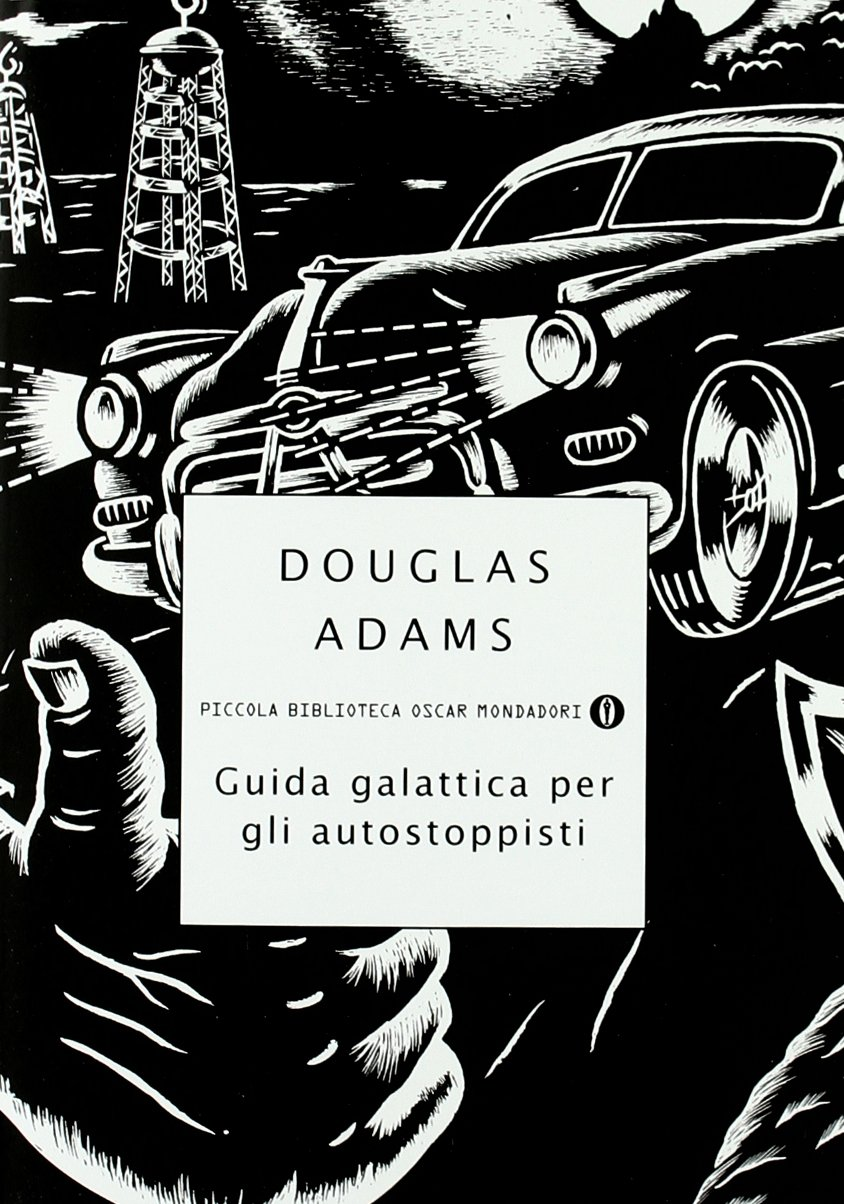
\includegraphics[scale=0.5]{res/img/immagine}
 \caption{Un'immagine bellissima.}
\end{figure}
\end{minted}
\end{code}
\end{esempio}


\end{frame}

\begin{frame}
 \frametitle{Ora il passo finale...}
 
 \huge Compiliamo!
 
 
 \begin{textblock*}{5cm}(6.5cm,3cm)
   
\includegraphics[scale=0.5]{icon-build}
 \end{textblock*}
\end{frame}
